\subsection{Understanding the PN junction and the Diode}\label{sec:pn_junction_diode}

Most explanations and graphics for this section are taken or inspired from the two brilliant explanation from \emph{The Organic Chemistry Tutor} Youtube Video "What is a Diode", and \emph{The Engineering Mindset} Video "Diodes Explained". The precise dynamics of what I am explaining could be studied over a whole semester, but understanding the basic idea is enough for what's needed from us in the exam. If you want more, refer to the Textbook, which will point you to appropriate electrostatics and semiconductor textbooks. \\

So, let's start. You might have heard of diodes before NE1 - they are semi-conductive devices that allow current to flow in one direction only. Ever heard of LEDs? Yes, they're diodes: Light Emitting Diodes. 

\begin{figure}[H]
    \centering
    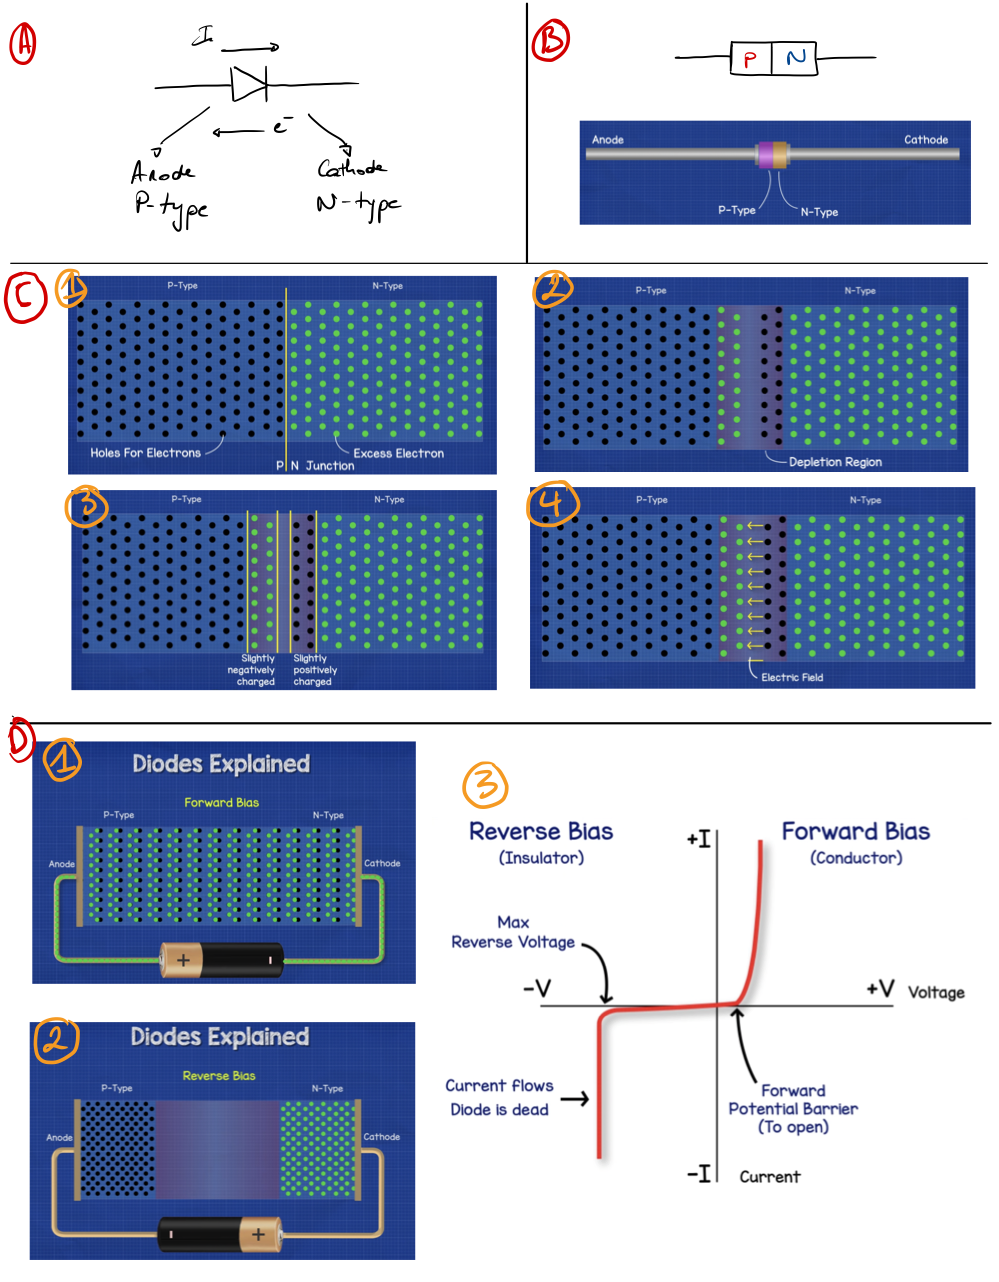
\includegraphics[width=1\linewidth]{../../Figures/Diode.png}
    \caption{Understanding the diode. A) Schematic of diode in circuit with its anode and cathode. B) Schematic representation of the structure of a diode, and its \textit{PN Junction}. C) What happens when sticking P-Type and N-Type semi conductor materials together. D) Forward and reverse current functionning principles in diodes. Adapted from multiple places.}
    \label{fig:diode}
\end{figure}

Diodes are drawn in circuits as shown on figure \ref{fig:diode}.A. Current flows in the direction of the arrow, which means that electrons flow in the opposite direction (thanks again Benjamin Franklin). The "wall" at the tip of the arrow is there to remind you that current really only flows in one direction. So how does it do it? How does it allow current to flow only in one direction? 

Diodes are essentially \textbf{PN Junctions}. A PN junction is what happens when you put P-Type doped semi conductor next to N-Type doped semi conductor (typically silicon). As shown in figure \ref{fig:diode}.B. the P-Type semi-conductor is known as the anode, and the N-type to an cathode. What happens when you stick P-Type and N-Type semi-conductors together? \\

This is the purpose of figure \ref{fig:diode}.C. As you already know, and as you can see in figure \ref{fig:diode}.C.1, the P-Type is filled with free holes and the N-Type is filled with free electrons. The junction between the two is what we call the \textit{PN Junction}. \ref{fig:diode}.C.1 only shows you what you theoretically expect, but of course, as soon as you actually stick the two bits together, things start happening, which are shown in \ref{fig:diode}.C.2-4. The first thing to consider is that some of the excess electrons from the N-Type move over to the P-type side to occupy some holes. This occurs in the \textbf{depletion region} that you see in \ref{fig:diode}.C.2. This causes some of the initially P-Type region to become slightly negatively charged and the N-type region to become slightly positively charged \ref{fig:diode}.C.3. This creates an \textit{electric field}, which prevents further electrons from moving across (\ref{fig:diode}.C.4). The depletion region is defined as \textit{a region in semiconductor devices, usually at the juncture of P-type and N-type materials, in which there is neither an excess of electrons nor of holes}. This works with our figure and explanations! 

In typical diodes, made of silicon, you should know that the potential difference between the slightly positive and slightly negative region is $\approx$ 0.7 Volts. This will become relevant soon.

Now what happens when you connect a voltage source to the diode? \\

This is the purpose of figure \ref{fig:diode}.D. If you connect the anode (P-type) to the positive end of your voltage source, and the cathode (N-type) to the negative end, you'll get (if the potential difference on your battery is $>0.7V$) a nice current flowing in \textbf{forward bias mode} (\ref{fig:diode}.D.1). Alternatively, if you reverse the power supply, for reasons that become very clear on \ref{fig:diode}.D.2, the holes are pulled towards the negative and electrons towards the positive, which causes the barrier to expand and (almost) no current to flow: we're in \textbf{reverse bias mode}. Yes, the barrier is similar to the band gaps we talked about before - and this is why in reverse bias mode, the diode acts as an insulator. We now know how diodes only allow current to flow in one direction. Pretty cool right? The stronger the reverse bias, the larger the surface area of the depletion region! This will be particularly relevant in the photodiode chapter. 
Now to enter a bit more details, which are shown in \ref{fig:diode}.D.3: current really starts flowing when you apply a voltage (in the right mode) superior to some "forward potential barrier", which in the case of silicon is $\approx$ 0.7V. From then, current flows. Now when we apply a voltage in reverse bias mode, you can see on \ref{fig:diode}.D.3 that the current flow is not exactly 0 (because it really never is anyways). If you apply a strong enough voltage in reverse bias (remember, voltage on Kryptonite), you eventually will force a current, and probably damage your diode by the same occasion (just like Superman would break the wall and not simply go through it). In general, you always have both a forward and reverse current component, that's just how electron dynamics work, though depending on the voltage you apply, one is several orders of magnitude more important than the other, which is why we often neglect it.

\paragraph{What does this give in Band Energy Diagrams?}
You thought you could escape it didn't you? Don't worry, we'll make it simple. 

\begin{figure}[H]
    \centering
    \includegraphics[width=0.95\linewidth]{../../Figures/PN Band Energy.png}
    \caption{Band diagram of the diode, and its corresponding electric field $\epsilon$ in the depletion region. Electric field is negative as it, by convention, is from positive to negative, and the arrow points from negative to positive. Adapted from multiple places.}
    \label{fig:Diode Band diagram}
\end{figure}


